\section{Introduction}
\label{sec:introduction}

eBPF now runs production networking, security, and observability inside the Linux kernel~\cite{gbadamosi2024ebpf}. Every program must first pass a static safety verifier, which rejects any program it cannot prove safe~\cite{gershuni2019simple}. When the verifier rejects a program, it returns a log of bytecode instructions and register states, ending in an error message. While the log records every step the verifier took, it is usually hard for a developer to tell why the program was rejected or what to change. As a result, the developer resorts to time-consuming trial and error to satisfy the verifier~\cite{deokar2024empirical}.

To identify the gap, we construct \empiricalset, a corpus of 235 rejections reproduced from real projects. We read each rejection's source and fix to assign the responsible layer: 191 are source bugs, and the other 44 are rejections of correct code, caused by the compiler, the environment, or the verifier. For the source bugs, we further classify the root cause into 12 categories. We find the verifier's log difficult to use for repair, for two reasons. First, it does not reveal the root cause: a single error message can arise from as many as seven root-cause categories. Second, it carries no field for the responsible layer. Tools that help developers read the verifier's output, such as PrettyVerifier~\cite{rizza2025design} and the BPF Verifier Visualizer~\cite{bpfvv}, enhance or visualize it but do not reconstruct the verifier's reasoning.

While the verifier's log lacks the two categories of information described above, a tool can recover them from the log to help diagnose and fix the program. The verifier builds a safety proof as it checks the program instruction by instruction, then discards the proof at the rejected operation and reports only the symptom. Under \texttt{log\_level=2}, though, it records its state after every instruction~\cite{linuxkernel-bpf-verifier,vishwanathan2022sound}. From these states, a tool reconstructs the discarded proof, which reveals the missing information.

To help a developer diagnose and fix a rejection, we introduce \sys, a userspace tool that turns the verifier's rejection log into a compiler-style diagnostic. Figure~\ref{fig:overview} shows \sys on a real rejection, where the verifier returns a single register-level line. From the same log, \sys maps the terminal message to the safety property the verifier could not prove. \sys then traces the property through the per-instruction states, recording where it is established and where it is lost. From the reconstructed proof, \sys renders a diagnostic that gives the root cause and the responsible layer.

We test whether the \sys diagnostic enables more repairs than the raw verifier log. We give a language model the buggy program with either the raw log or the \sys diagnostic, on \bench, a suite of 75 repair tasks, each checked by an executable oracle independent of \sys~(\S\ref{sec:evaluation}). Replacing the raw log with the diagnostic raises one-shot repair under all three models we test. On Qwen3.6 27B, the model repairs 22 of the 75 cases from the raw log and 38 from the diagnostic.

This paper makes the following contributions:
\begin{itemize}
\item We conduct an empirical study on \empiricalset to identify the gap between the verifier's log and a repair.
\item We build \sys, a tool that recovers the root cause and responsible layer from the verifier's discarded proof.
\item We build two datasets: \empiricalset, a corpus of 235 reproduced rejections for the empirical study, and \bench, 75 repair tasks with executable oracles for evaluating repair.
\end{itemize}

\begin{figure}[t]
  \centering
  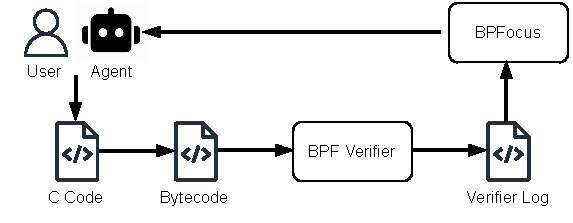
\includegraphics[width=0.96\columnwidth]{figures/sec-1-overview.pdf}
  \vspace{0.5pt}

  \noindent\textbf{\footnotesize (a) C Code}
  \begin{lstlisting}[style=bpfix,language=C,firstnumber=263]
if (ipv4_hdr)
    udph = (void *)ipv4_hdr + sizeof(*ipv4_hdr);
else
    udph = (void *)ipv6_hdr + sizeof(*ipv6_hdr);
if (udph + sizeof(struct udphdr) > data_end)  // bounds-checked
    return 1;

dst_port = __constant_ntohs(((struct udphdr *)udph)->dest); // rejected
  \end{lstlisting}

  \noindent\textbf{\footnotesize (b) Verifier Log}
  \begin{lstlisting}[style=bpflog]
from 31 to 34: ... R5_w=40 ...
; if (udph + sizeof(struct udphdr) > data_end) @ prog.c:267
35: (07) r3 += 8                      ; R3=48
36: (2d) if r3 > r2 goto pc+4         ; R2=pkt_end() R3=48
; dst_port = ...((struct udphdr *)udph)->dest; @ prog.c:270
37: (69) r2 = *(u16 *)(r5 +2)
R5 invalid mem access 'scalar'
  \end{lstlisting}

  \noindent\textbf{\footnotesize (c) \sys output}
  \begin{lstlisting}[style=bpfdiag]
error[BPFOCUS-E006]: verifier-visible compiler lowering hides the required proof
  = class: lowering_artifact
  = confidence: medium
  = next action: provenance
  --> prog.c:270
   |
263 | if (ipv4_hdr)
    | ------------- nearby source context for pointer provenance
267 | if (udph + sizeof(struct udphdr) > data_end)
    | -------------------------------------------- verifier state changes from pkt to scalar before the rejected access
270 | dst_port = __constant_ntohs(((struct udphdr *)udph)->dest);
    | ^^^^^^^^^^^^^^^^^^^^^^^^^^^^^^^^^^^^^^^^^^^^^^^^^^^^^^^^^^^ rejected here: verifier sees a scalar where a pointer is required
   |
   = verifier[229]: R5 invalid mem access 'scalar'
   = required proof: preserve a verifier-recognized pointer type at the operation that requires a pointer
help: Reacquire a verifier-tracked pointer before the rejected dereference.
help: Use the packet pointer that received the data_end proof, or rederive and recheck it before the load.
  \end{lstlisting}
  \caption{\sys on a real rejection (Stack Overflow 53136145). The verifier returns one register-level line; from the same log, \sys reconstructs the discarded proof and localizes the rejection to the point where the required proof was lost, mapping each span back to source.}
  \label{fig:overview}
\end{figure}
